\chapter{Theoretical Background}
\section{Transformers}
        A transformer model is a neural network that learns context and thus meaning by tracking relationships in sequential data like the words in this sentence.
        Transformer models apply an evolving set of mathematical techniques, called attention or self-attention, to detect subtle ways even distant data elements in a series influence and depend on each other.
        First described in a 2017 paper from Google\cite{vaswani2023attention}, transformers are among the newest and one of the most powerful classes of models invented to date. They’re driving a wave of advances in machine learning some have dubbed transformer AI.
        Stanford researchers called transformers “foundation models” in an August 2021 paper\cite{bommasani2021opportunities} because they see them driving a paradigm shift in AI.

        \begin{figure}[hbt!]
            \center{
                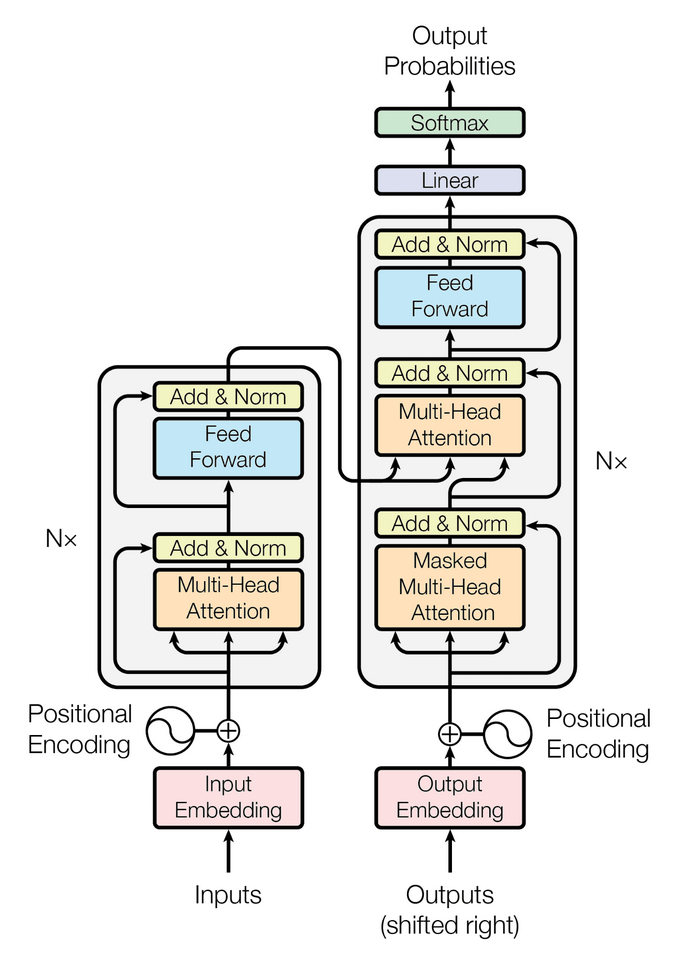
\includegraphics[width=0.46\textwidth]{./img/attention_research_1.png}
                \caption{The Transformer - model architecture.\cite{vaswani2023attention}}
                }
        \end{figure}

\section{BERT}
    BERT stands for Bidirectional Encoder Representations from Transformers. It is designed to train deep bidirectional representations from unlabeled text by jointly conditioning on both left and right context \cite{devlin2019bert}. BERT utilizes the Transformer architecture, which employs an attention mechanism to understand contextual relationships among words or sub-words within a text. The basic Transformer structure consists of two distinct components: an encoder, which processes the input text, and a decoder, which generates predictions for the given task. BERT architecture enables it to handle various NLP tasks effectively, such as question answering, sentiment analysis, and text classification, by fine-tuning on specific datasets. 

    \begin{figure}[hbt!]
        \center{
            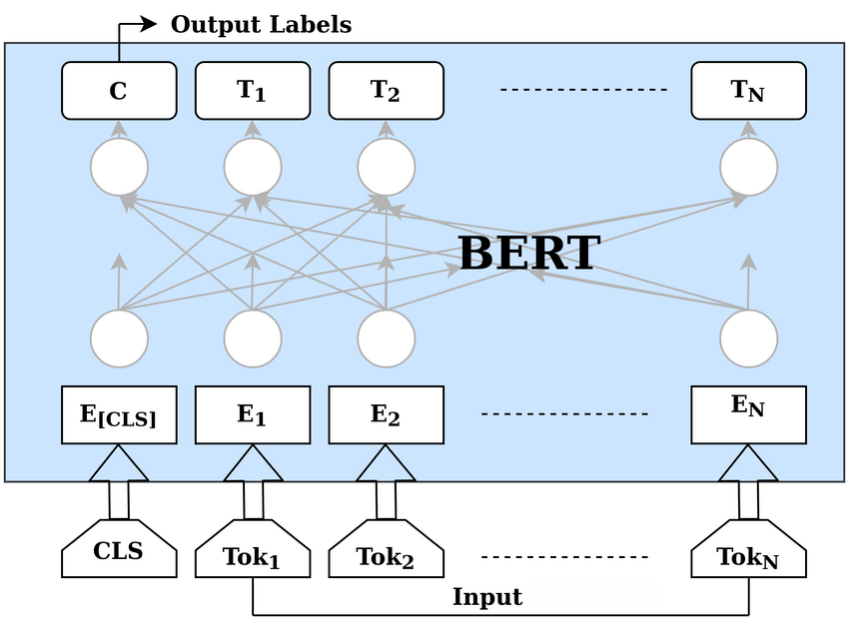
\includegraphics[width=1\textwidth]{./img/bertarchitecture.png}
            \caption{Illustrations of Fine-tuning BERT on Different Tasks.\cite{Gundapu}}
            }
    \end{figure}
